\section{Theory}
\label{sec:Theory}
% Delaunay-triangulering, punktsett, sirkelkriterie, distmesh (ikke 3D), etc.
This project is a continuation on previous work by \textcite{UPR_thesis}, and most of the theory in this section is, unless otherwise stated, based on \textcite{UPR_thesis} or \textcite{UPR_chapter}.

To produce and use discrete representations of the real world, there must be a way to map the real, continuous domain to a discrete representation. This is typically done by looking at a set of points in the real domain.

\begin{definition}[Point set]
A point set $P \in \mathbb{R}^n$ is a finite set of points in $\mathbb{R}^n$.
\end{definition}
While there exist infinite point sets, we limit ourselves to finite sets in order to have a discrete representation. To encode more data in the discrete representation, points in a point set can be grouped into simplices. This enables the inclusion of data about physical properties such as subsurface faults, wells and other geological features, which are necessary for accurate simulations. Using simplices to represent a domain enables us to reduce the amount of data necessary for representing a domain with physical features, compared to using a large point set to represent the domain.


\begin{definition}[Simplex]
A simplex is a generalization of a triangle to arbitrary dimensions.
\end{definition}
Simplices represent the simplest possible geometric object in a space. As discrete representations of objects in physical space are limited to at most three spatial dimensions, we only need to consider the first four simplices (Figure~\ref{fig:simplices}):
\begin{itemize}
    \item A 0-simplex is a point.
    \item A 1-simplex is a line.
    \item A 2-simplex is a triangle.
    \item A 3-simplex is a tetrahedron.
\end{itemize}

\begin{figure}[ht]
    \centering
    \begin{subfigure}[b]{0.2\textwidth}
        \centering
        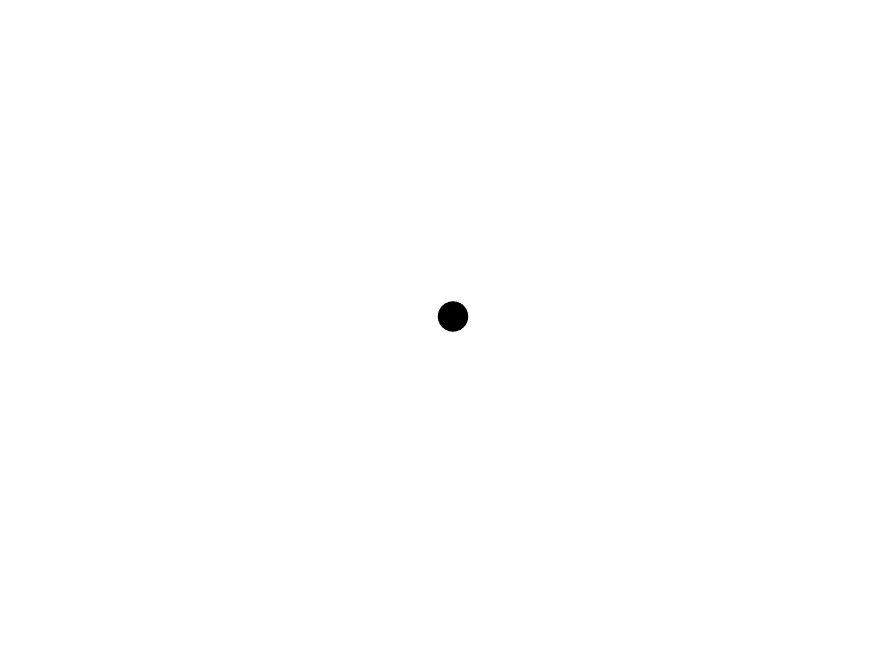
\includegraphics[width=\textwidth]{report/Images/Theory/simplices/simplices0.png}
        \caption{0-simplex}
        \label{fig:0-simplex}
    \end{subfigure}
    \hfill
    \begin{subfigure}[b]{0.2\textwidth}
        \centering
        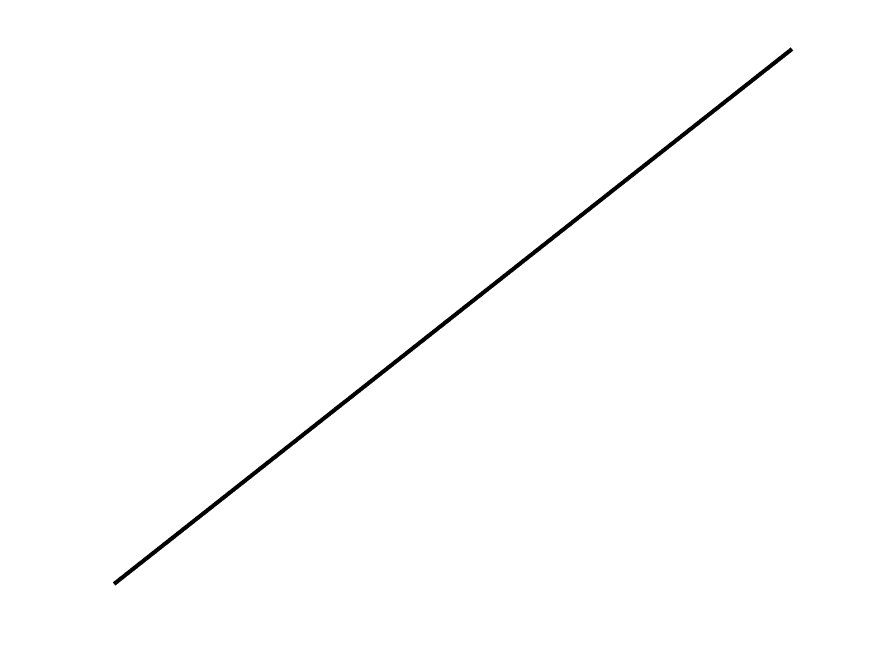
\includegraphics[width=\textwidth]{report/Images/Theory/simplices/simplices1.png}
        \caption{1-simplex}
        \label{fig:1-simplex}
    \end{subfigure}
    \hfill
    \begin{subfigure}[b]{0.2\textwidth}
        \centering
        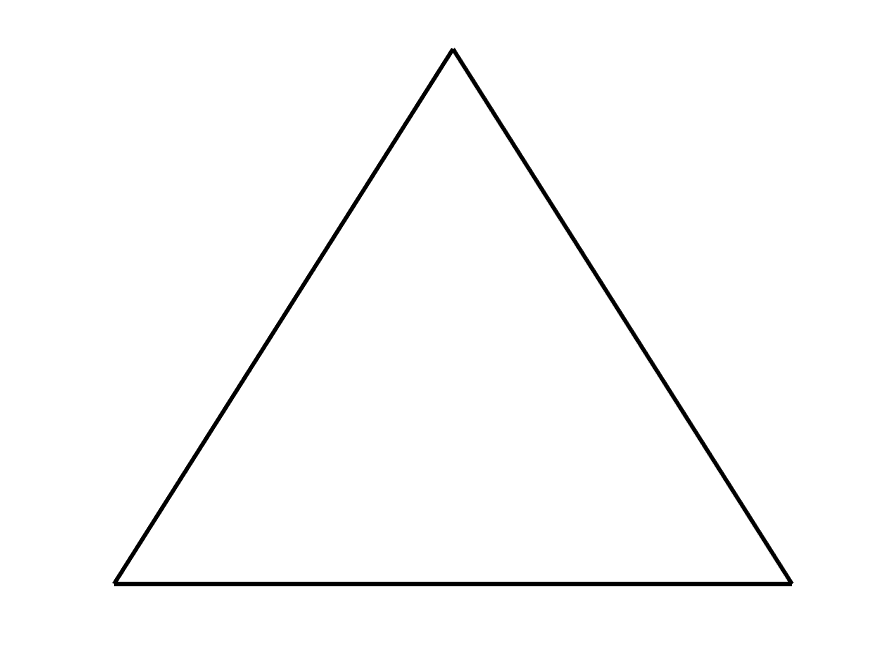
\includegraphics[width=\textwidth]{report/Images/Theory/simplices/simplices2.png}
        \caption{2-simplex}
        \label{fig:2-simplex}
    \end{subfigure}
    \hfill
    \begin{subfigure}[b]{0.2\textwidth}
        \centering
        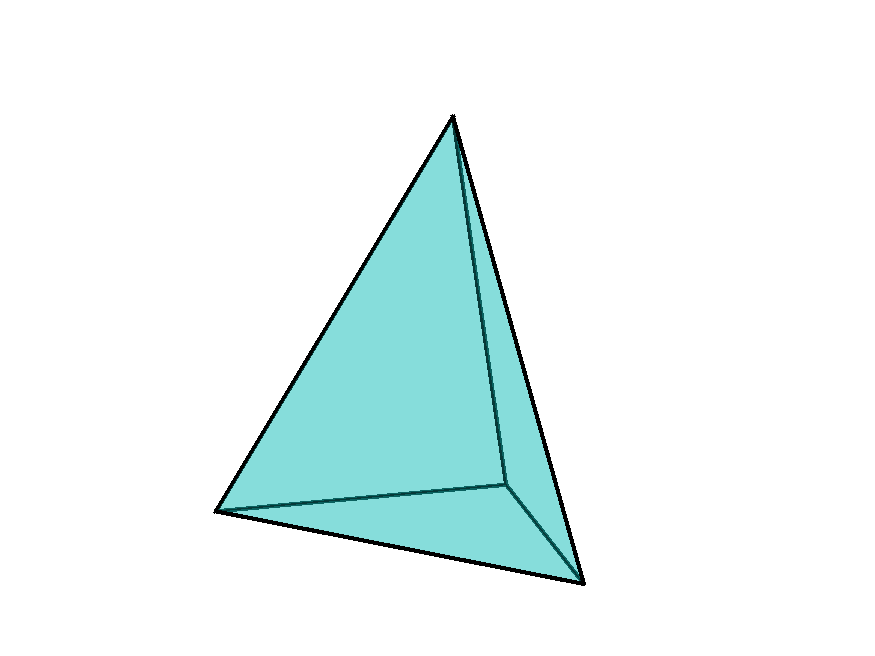
\includegraphics[width=\textwidth]{report/Images/Theory/simplices/simplices3.png}
        \caption{3-simplex}
        \label{fig:3-simplex}
    \end{subfigure}
    \hfill
    \caption{Illustration of the first 4 simplices.}
    \label{fig:simplices}
\end{figure}

In general, a $k$-simplex is a $k$-dimensional geometric object consisting of the \emph{convex hull} of its $k + 1$ vertices.


\begin{definition}[Convex hull]
The convex hull of a point set $P$ is the minimal convex set containing $P$.
\end{definition}
\begin{figure}[ht]
    \centering
    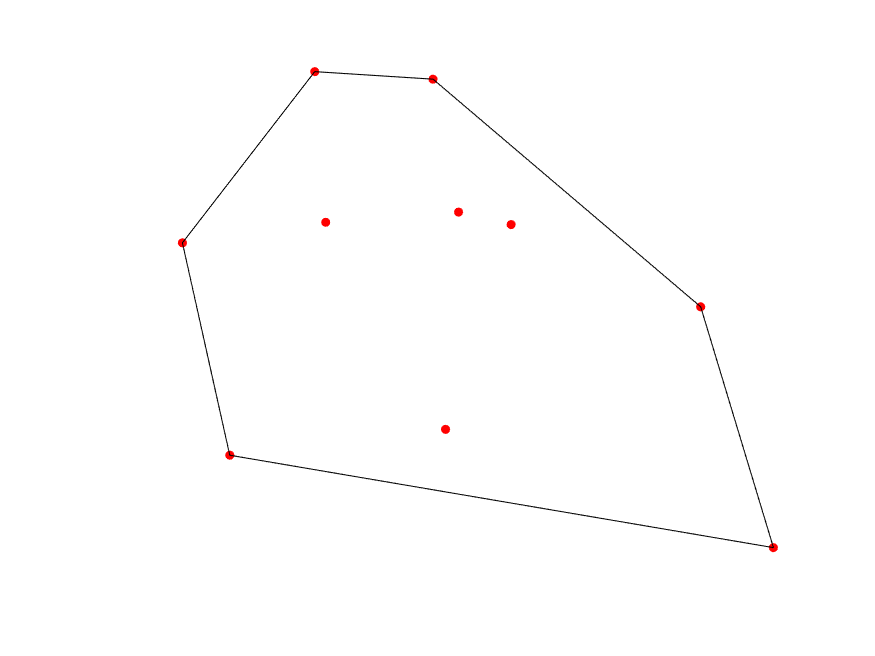
\includegraphics[width=0.5\textwidth]{report/Images/Theory/convex_hull.png}
    \caption[Example of a convex hull]{Example of a convex hull for a set of 10 randomly generated points in $\mathbb{R}^2$.}
    \label{fig:ex:convex_hull}
\end{figure}

The process of converting a point set into a set of simplices is called \emph{triangulation}.

\begin{definition}[Triangulation]
A triangulation $T$ of a point set $P$ is the set of simplices $T$ such that:
\begin{itemize}
    \item the set of vertices in $T$ equals $P$, and
    \item the union of all simplices in $T$ equals the convex hull of $P$, i.e., the union of all simplices in $T$ makes up the minimal convex set containing $P$.
\end{itemize}
\end{definition}
\begin{figure}[ht]
    \centering
    \begin{subfigure}[b]{0.4\textwidth}
        \centering
        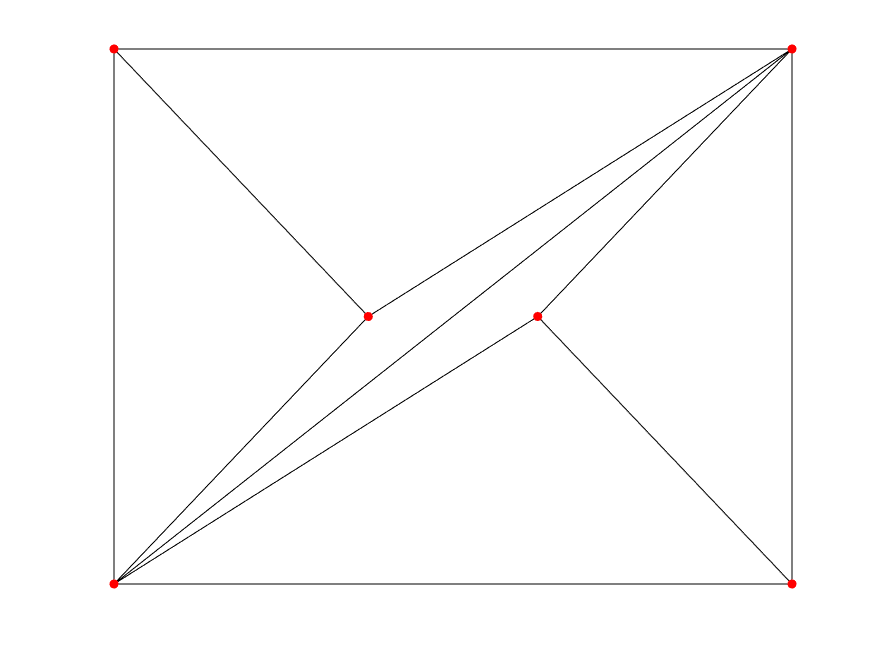
\includegraphics[width=\textwidth]{report/Images/Theory/triangulation/triangulation_random.png}
        \caption{Random triangulation}
        \label{fig:triangulation-random}
    \end{subfigure}
    \begin{subfigure}[b]{0.4\textwidth}
        \centering
        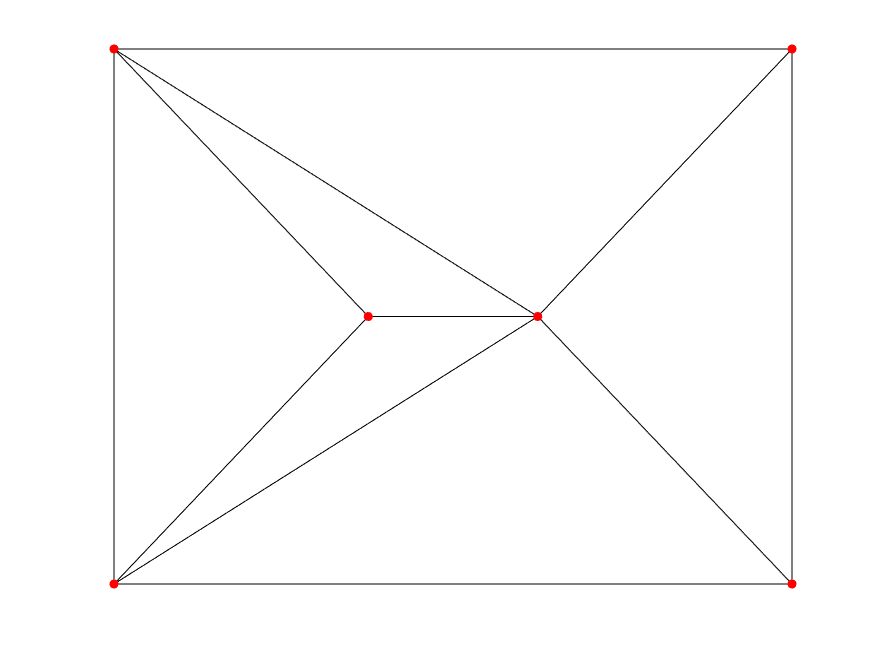
\includegraphics[width=\textwidth]{report/Images/Theory/triangulation/triangulation_delaunay.png}
        \caption{Delaunay triangulation}
        \label{fig:triangulation-delaunay}
    \end{subfigure}
    \caption[Example of triangulation]{Example of two triangulations for a set of points $P \in \mathbb{R}^2$.}
    \label{fig:ex:triangulation}
\end{figure}

For a given point set, one can generally create multiple valid triangulations. \autoref{fig:ex:triangulation} shows two triangulations for the same point set $P$.


\subsection{Delaunay triangulation}
Delaunay triangulations were first introduced by \textcite{delaunay_1943} in 1943. Delaunay triangulations maximize the smallest angle of the simplices in the triangulation and therefore produce representations that work nicely in grid-based applications. The Delaunay triangulation of a point set $P$ is defined as follows:
\begin{definition}
\label{def:delaunay}
The $T$ triangulation of the point set $P$ is a Delaunay triangulation if no vertices in $P$ are inside the \emph{circumcircle} of any simplex in $T$.
\end{definition}

\begin{definition}[Circumcircle]
A circumcircle of a polygon is a circle passing through all vertices of the polygon. The circumcircles of a triangulation is the set of circumcircles of all simplices in the triangulation.
\end{definition}

\begin{figure}[ht]
    \centering
    \begin{subfigure}[b]{0.4\textwidth}
        \centering
        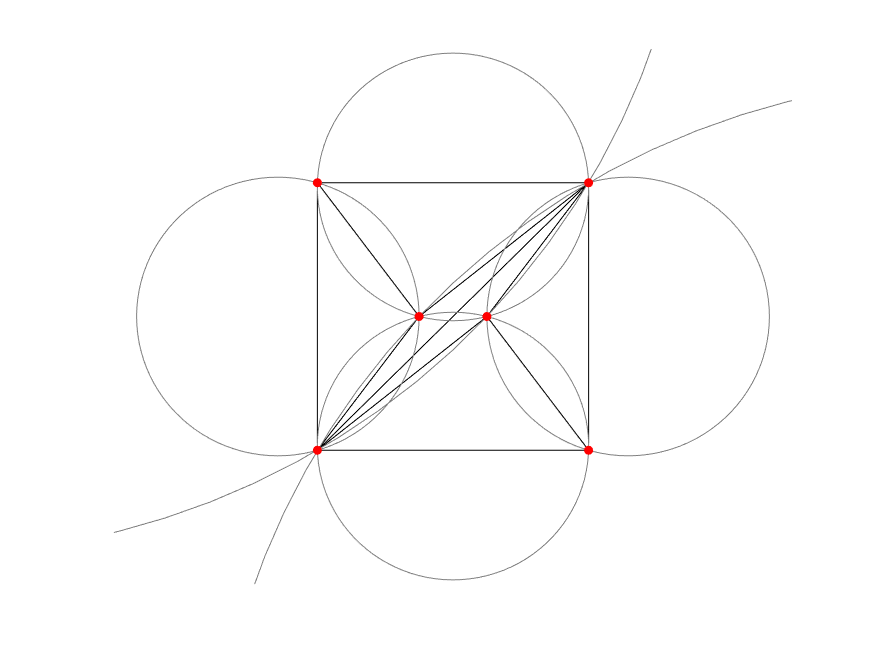
\includegraphics[width=\textwidth]{report/Images/Theory/circumcircles/circumcircle_random.png}
        \caption{Circumcircles of \autoref{fig:triangulation-random}}
        \label{fig:circumcircles-random}
    \end{subfigure}
    \begin{subfigure}[b]{0.4\textwidth}
        \centering
        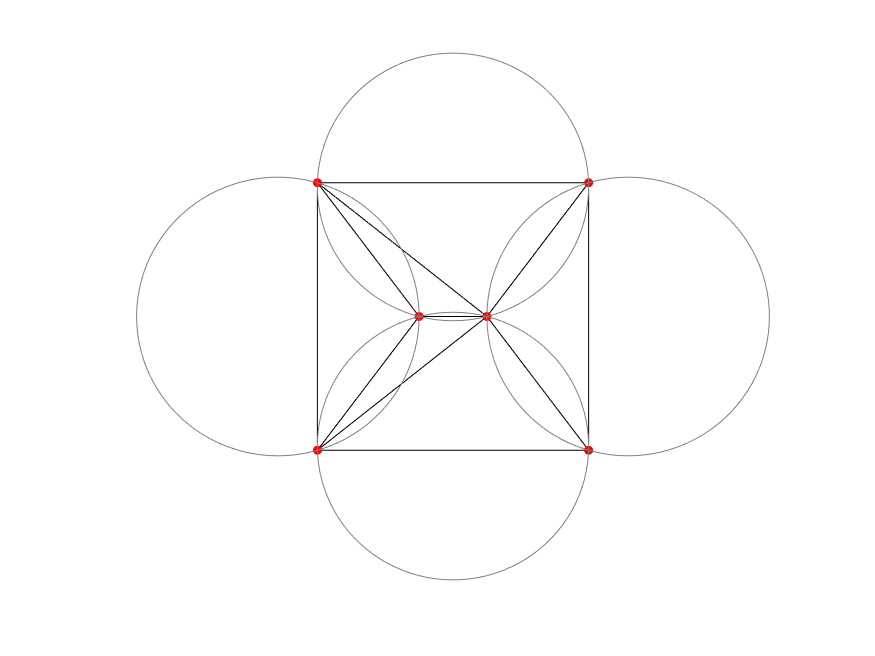
\includegraphics[width=\textwidth]{report/Images/Theory/circumcircles/circumcircle_delaunay.png}
        \caption{Circumcircles of \autoref{fig:triangulation-delaunay}}
        \label{fig:circumcircles-delaunay}
    \end{subfigure}
    \caption[Example of circumcircles]{Example of circumcircles for the two triangulations in \autoref{fig:ex:triangulation}. Note that \autoref{fig:circumcircles-random} has a been cropped so that two of the circumcircles are only shown as arcs.}
    \label{fig:ex:circumcircles}
\end{figure}


In \autoref{fig:circumcircles-delaunay}, no vertices of $P$ are inside any of the plotted circumcircles. This shows that the triangulation in \autoref{fig:triangulation-delaunay} is a Delaunay triangulation. In \autoref{fig:circumcircles-random}, two vertices are inside each of the two large circumcircles created from the centermost, obtuse triangles. This shows that the triangulation in \autoref{fig:triangulation-random} is not Delaunay.

Delaunay triangulations are unique as long as at most three vertices are on the same circumcircle \cite[Theorem 2.1]{UPR_thesis}. In cases where this is not true, such as where four vertices make up a cyclic quadrilateral, there exist several valid Delaunay triangulations for the same point set $P$. This is illustrated in \autoref{fig:non-unique-delaunay}, where the two center vertices make up cyclic quadrilaterals with both the top and bottom pair of vertices. This enables four valid Delaunay triangulations of the point set.

\begin{figure}[ht]
    \centering
    \begin{subfigure}[b]{0.2\textwidth}
        \centering
        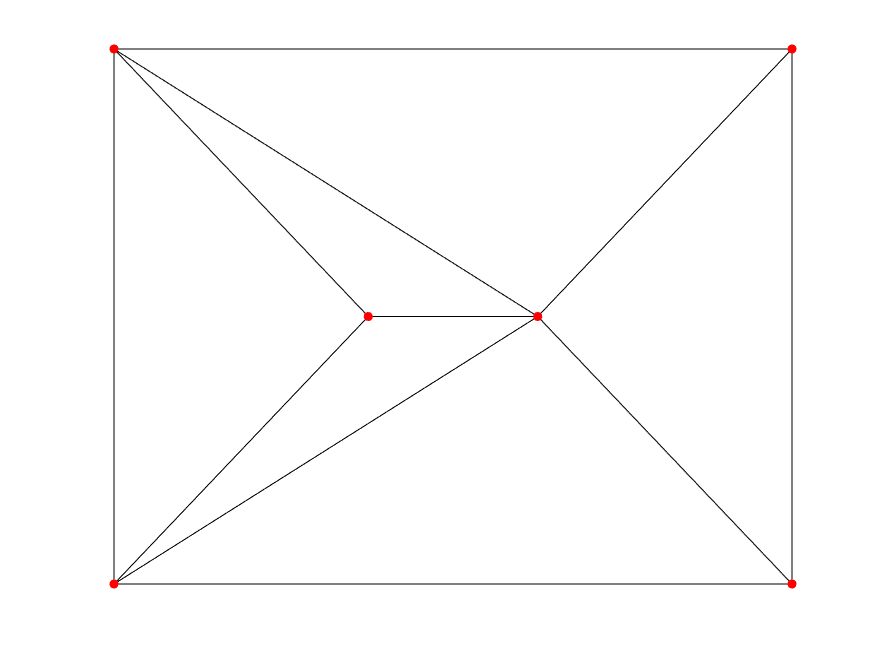
\includegraphics[width=\textwidth]{report/Images/Theory/triangulation/triangulation_delaunay.png}
        \label{fig:triangulation-delaunay1}
    \end{subfigure}
    \hfill
    \begin{subfigure}[b]{0.2\textwidth}
        \centering
        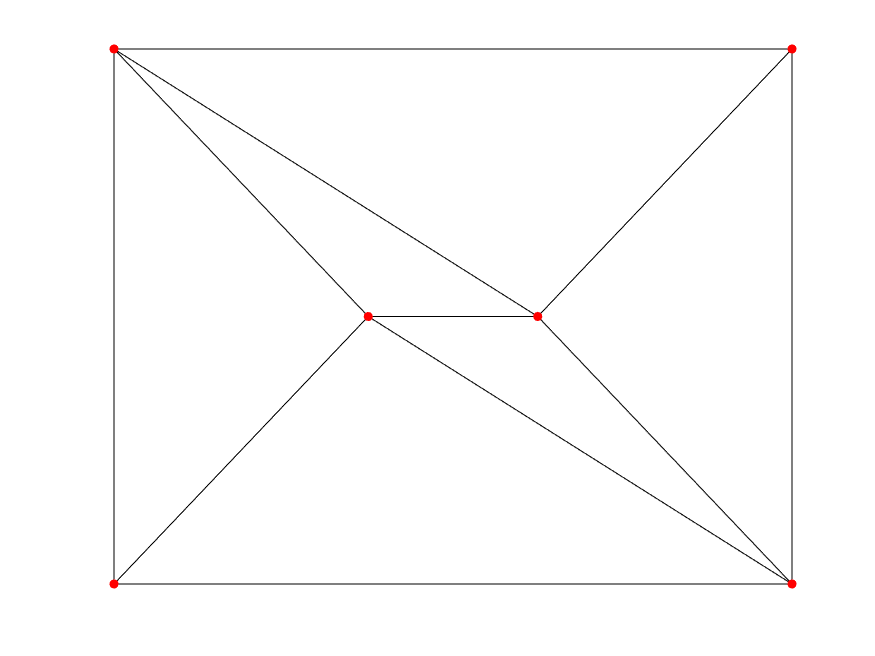
\includegraphics[width=\textwidth]{report/Images/Theory/triangulation/triangulation_delaunay3.png}
        \label{fig:triangulation-delaunay3}
    \end{subfigure}
    \hfill
    \begin{subfigure}[b]{0.2\textwidth}
        \centering
        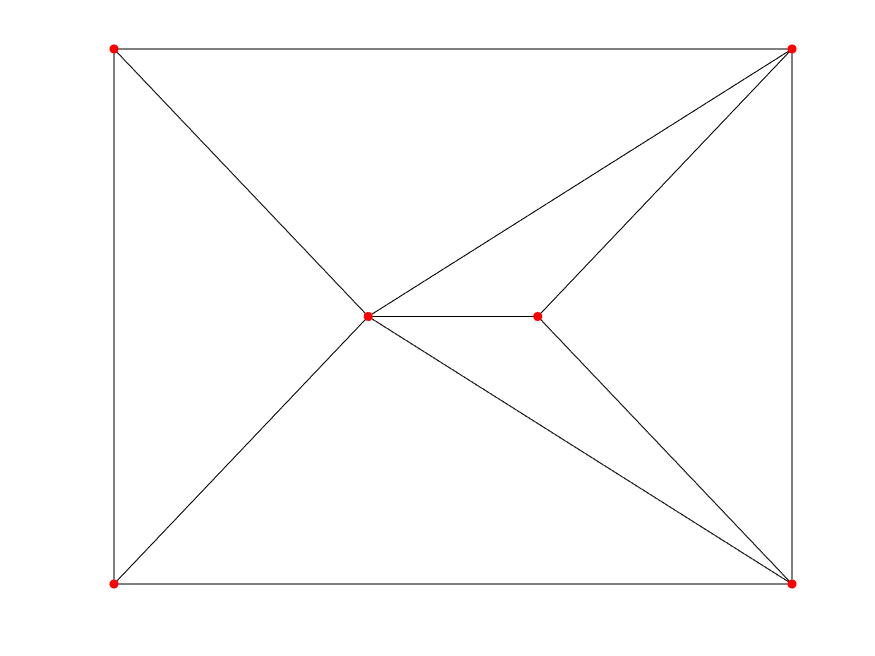
\includegraphics[width=\textwidth]{report/Images/Theory/triangulation/triangulation_delaunay2.png}
        \label{fig:triangulation-delaunay2}
    \end{subfigure}
    \hfill
    \begin{subfigure}[b]{0.2\textwidth}
        \centering
        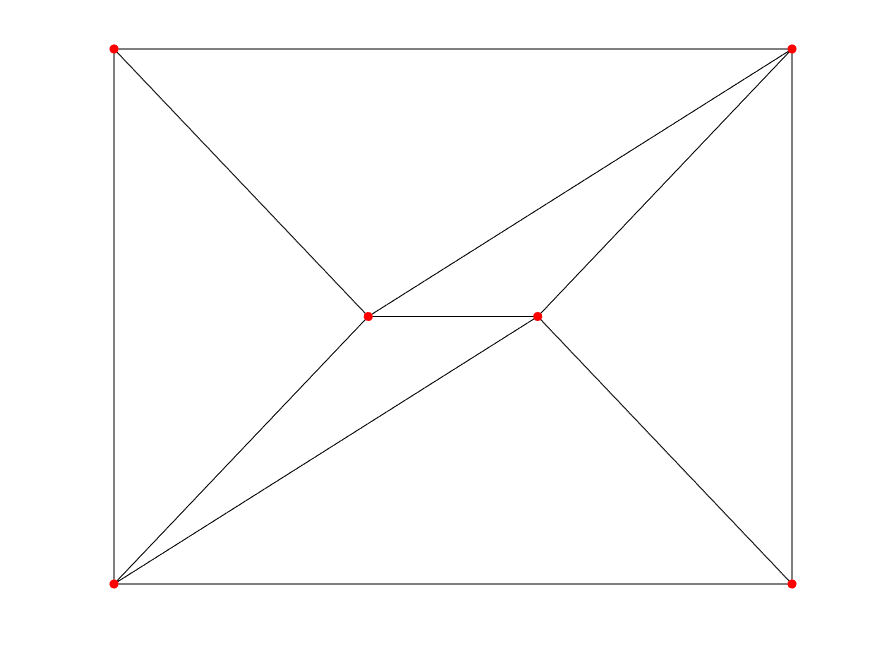
\includegraphics[width=\textwidth]{report/Images/Theory/triangulation/triangulation_delaunay4.png}
        \label{fig:triangulation-delaunay4}
    \end{subfigure}
    \caption[Non-uniqueness of Delaunay triangulations]{Non-uniqueness of Delaunay triangulations. Two cyclic quadrilaterals enable four valid Delaunay triangulations.}
    \label{fig:non-unique-delaunay}
\end{figure}



\subsection{Voronoi diagrams}
A \emph{Voronoi diagram} is a form of gridding formally introduced by \textcite{VoronoiNouvellesAD}, which is closely related to Delaunay triangulations. 

\begin{definition}[Voronoi diagram]
\label{def:voronoi}
Let $P$ be a point set in $\mathbb{R}^n$ consisting of points $p_i \in P$ for $i = 1,\dots,m$. Each point $p_i$ is called a \emph{site}. A point $x \in \mathbb{R}^n$ belongs to the \emph{Voronoi cell} $v_i$ associated with point $p_i$ if the distance between $p_i$ and $x$ is equal to the minimum distance from $x$ to any point $p \in P$. Formally, we can define this as
\begin{equation}
    v_i = \left\{ x : x \in \mathbb{R}^n \text{ s.t. } \abs{x - p_i} \leq \abs{x - p}\quad \forall p \in P \right\}.
\end{equation}
The set of all Voronoi cells $v_i$ is called a \emph{Voronoi diagram} or \emph{grid}.
\end{definition}

\begin{figure}[ht]
    \centering
    \begin{subfigure}[b]{0.3\textwidth}
        \centering
        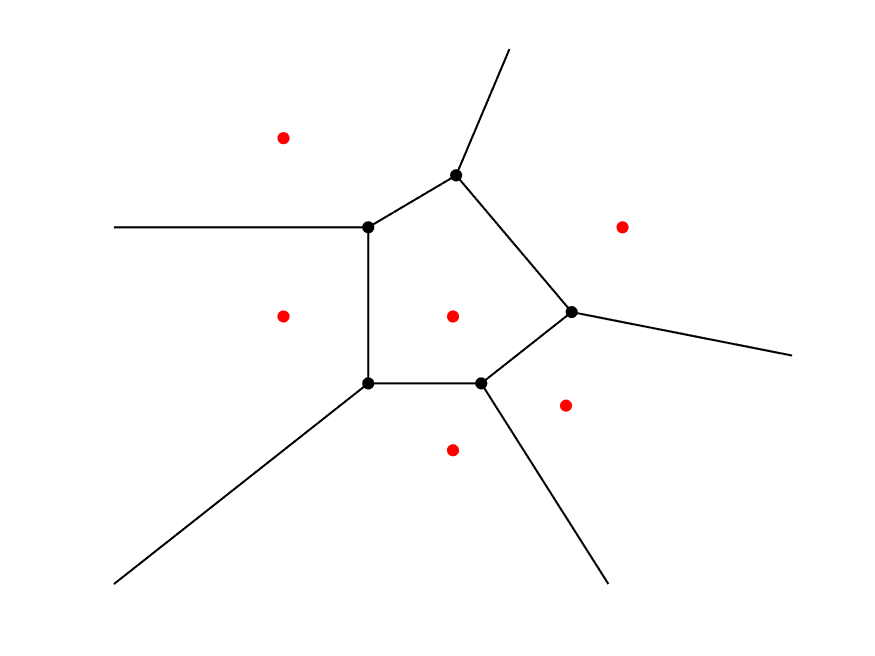
\includegraphics[width=\textwidth]{report/Images/Theory/voronoi/voronoi_example2.png}
    \end{subfigure}
    \begin{subfigure}[b]{0.3\textwidth}
        \centering
        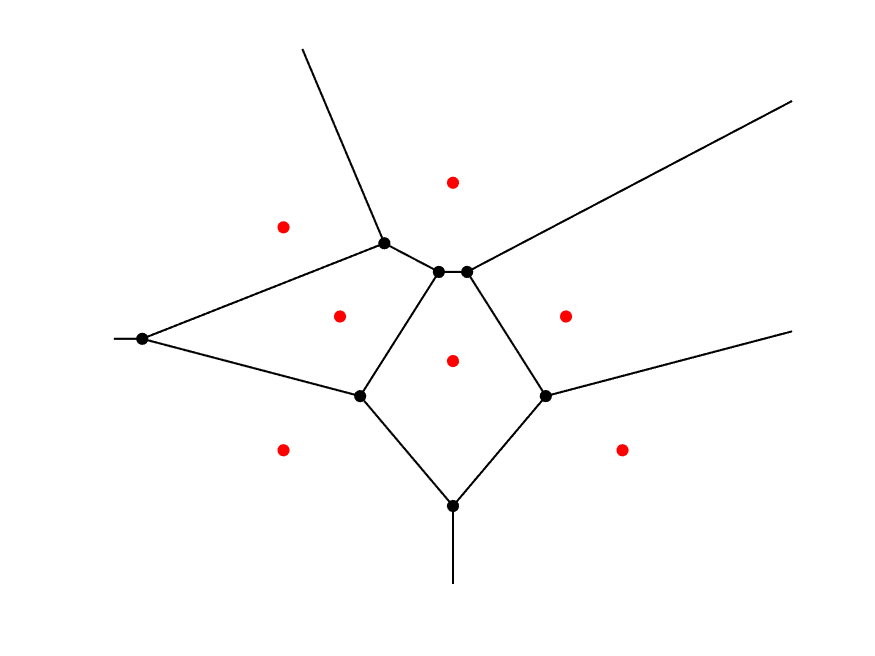
\includegraphics[width=\textwidth]{report/Images/Theory/voronoi/voronoi_example1.png}
    \end{subfigure}
    \begin{subfigure}[b]{0.3\textwidth}
        \centering
        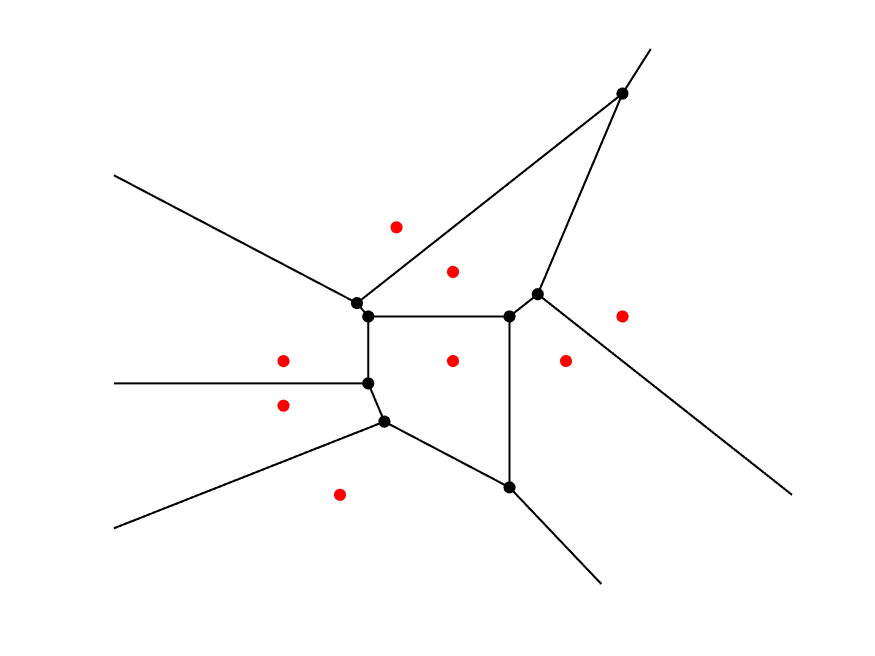
\includegraphics[width=\textwidth]{report/Images/Theory/voronoi/voronoi_example3.png}
    \end{subfigure}
    \caption[Example of Voronoi diagrams]{Example of Voronoi diagrams for different point sets, marked in red.}
    \label{fig:ex:only-voronoi}
\end{figure}

The intersection between two Voronoi cells $v_i$ and $v_j$ is called a face, and is denoted by $v_{i,j}$ \cite{UPR_chapter}. The face is made up of all points $x \in \mathbb{R}^n$ that are the same distance from $p_i$ and $p_j$, and where this distance is the same as the minimum distance from $x$ to any $p \in P$. We can define this formally as
\begin{equation}
\label{eq:voronoi-face}
    v_{i, j} = \left\{ x : x \in \mathbb{R}^d \text{ s.t. } \abs{x - p_i} = \abs{x - p_j} \leq \abs{x - p}\quad \forall p \in P \right\}.
\end{equation}

We can, in general, say that a $k$-face of a Voronoi diagram is the $k$-dimensional intersection between Voronoi cells \cite{UPR_chapter}. We can define this formally as
\begin{equation}
\label{eq:voronoi-k-faces}
    v_{i,\dots, j} = \left\{ x : x \in \mathbb{R}^d \text{ s.t. } \abs{x - p_i} = \dots = \abs{x - p_j} \leq \abs{x - p}\quad \forall p \in P \right\}.
\end{equation}

When dealing with a two-dimensional domain, i.e., $P \in \mathbb{R}^2$, there are 1-dimensional faces as edges where two cells meet and 0-dimensional faces as vertices where two or more edges intersect. In \autoref{fig:ex:only-voronoi}, the 1-dimensional faces are marked by lines, and the 0-dimensional faces are marked by black dots. When $P \in \mathbb{R}^3$, we have 2-dimensional faces as planes where two 3-dimensional cells meet, 1-dimensional faces as edges where two planes intersect, and 0-dimensional faces as vertices where two or more edges intersect.

From \autoref{eq:voronoi-k-faces}, it follows that 0-dimensional faces, i.e., Voronoi vertices, are points where the distance to three Voronoi sites are equal and smaller than the distance to any other sites. We formalize this is \autoref{theorem:voronoi-vertex}.

\begin{theorem}
\label{theorem:voronoi-vertex}
Sites $p_i$, $p_j$ and $p_k \in P$ create a vertex $v_{i, j, k}$ if and only if the open circle intersecting all sites is empty of any sites in $P$. 
\end{theorem}
\begin{proof}
Let $C$ be the open circle intersecting $p_i$, $p_j$ and $p_k$, with radius $r$. Assume there is a site $p \in C$. Let $x$ be the center of $C$, i.e. the point where $\abs{x - p_i} = \abs{x - p_j} = \abs{x - p_k} = r$. As $p \in C$ and $C$ is an open circle, we have
\begin{equation*}
    \abs{x - p} < r = \abs{x - p_i} = \abs{x - p_j} = \abs{x - p_k}.
\end{equation*}
As $p \in P$, \autoref{eq:voronoi-k-faces} leads to $v_{i, j, k} = \emptyset$.
\end{proof}
The same holds true in $\mathbb{R}^3$, where four sites have a 0-dimensional face (vertex) if and only if the open ball intersecting all four sites is empty of any sites in $P$.

\subsubsection{Relationship between Delaunay and Voronoi}
\autoref{theorem:voronoi-vertex} appears to be very similar to the definition of Delaunay triangulation in Definition \ref{def:delaunay}. In fact, Delaunay triangulations and Voronoi grids are considered \emph{dualities} \cite{UPR_chapter}.

% \begin{definition}[Dualities]
% Dualities are two objects that have a one-to-one relationship, and can be translated back and forth.
% \end{definition}

Let $T$ be a Delaunay triangulation and $V$ be a Voronoi diagram, both on the same point set. Then each node in $T$ is associated with a cell in $V$, and vice versa. More specifically, the centers of the circumcircles used to prove $T$ is Delaunay are vertices in the Voronoi diagram, and if there is an edge in $T$ between two sites, then the sites share a face in $V$. Likewise, the sites in the Voronoi diagram are vertices in the Delaunay triangulation. This is illustrated in \autoref{fig:ex:voronoi}: sites are marked by blue dots and the circumcenters of the Delaunay triangulation are marked by red dots.\looseness=-1


\begin{figure}[ht]
    \centering
    \begin{subfigure}[b]{0.4\textwidth}
        \centering
        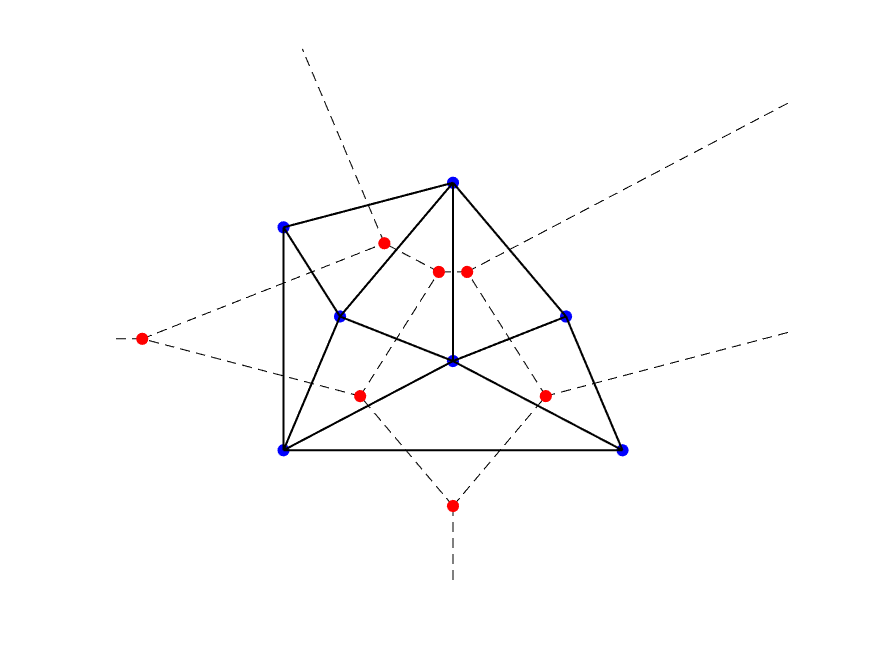
\includegraphics[width=\textwidth]{report/Images/Theory/voronoi/voronoi_duality_delaunay.png}
        \caption{Delaunay triangulation}
        \label{fig:ex:voronoi-delaunay}
    \end{subfigure}
    \begin{subfigure}[b]{0.4\textwidth}
        \centering
        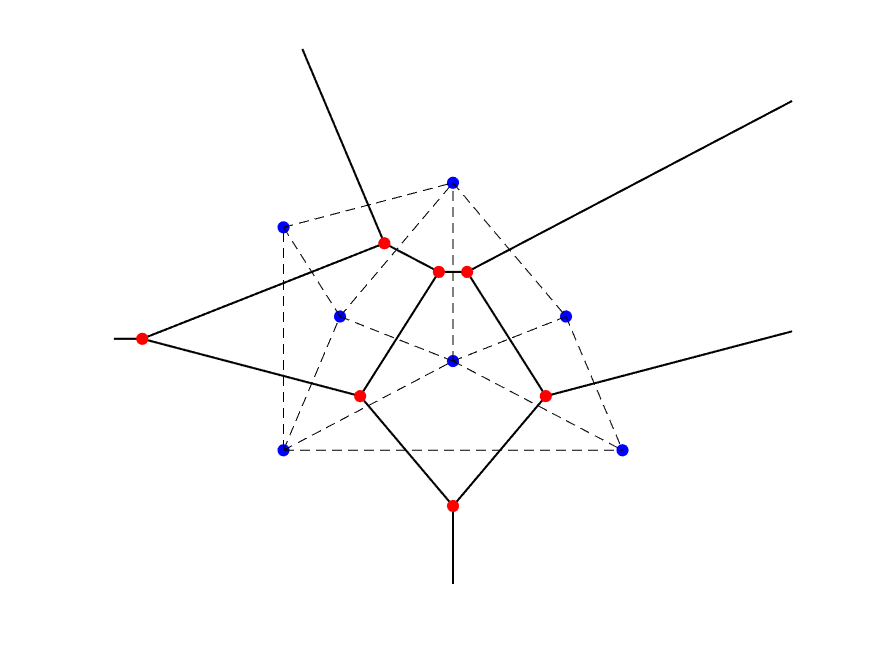
\includegraphics[width=\textwidth]{report/Images/Theory/voronoi/voronoi_duality_voronoi.png}
        \caption{Voronoi diagram}
        \label{fig:ex:voronoi-voronoi}
    \end{subfigure}
    \caption[Duality of Delaunay triangulations and Voronoi diagrams]{Delaunay triangulation and Voronoi diagram for the same point set.}
    \label{fig:ex:voronoi}
\end{figure}

\subsubsection{Clipped Voronoi diagrams}
One important, but in our case unwanted, property of Voronoi diagrams is that they extend to infinity. This is visible in both \autoref{fig:ex:only-voronoi} and \autoref{fig:ex:voronoi}. As we are interested in mapping real-world objects to discrete domains that can be used for simulations, infinite domains are unwanted. To handle this, we can limit the definition of Voronoi diagrams slightly, by creating \emph{clipped Voronoi diagrams}.

\begin{definition}[Clipped Voronoi diagram]
Let $P$ be a point set in a bounded domain $\mathcal{D} \subset \mathbb{R}^n$. We define a clipped Voronoi diagram as the set of all cells $v_i$, where
\begin{equation}
\label{eq:clipped-voronoi}
    v_i = \left\{ x : x \in \mathcal{D}\subset \mathbb{R}^n \text{ s.t. } \abs{x - p_i} \leq \abs{x - p}\quad \forall p \in P \right\}.
\end{equation}
\end{definition}

While there is little difference between clipped and unclipped Voronoi diagrams, limiting the domain is beneficial for simulations and computer representation.

\subsubsection{Centroidal Voronoi diagrams}
\label{sec:CVD}
The properties of a Voronoi diagram depend on the distribution of its sites. One especially interesting case happens when the sites and centers of each cell align. We use the mass center of the Voronoi cells to calculate this. The mass center of a Voronoi cell is given as
\begin{equation}
    \mathbf{c}_i = \frac
        {\int_{V_i} \mathbf{y} \rho(\mathbf{y}) d\mathbf{y}}
        {\int_{V_i} \rho(\mathbf{y}) d\mathbf{y}},
\end{equation}
where $V_i$ is the volume of the cell and $\rho(\mathbf{y})$ is a given mass density function of the cell. If the mass centers and sites in a Voronoi diagram line up, we have a special subset of Voronoi diagrams called a \emph{centroidal Voronoi diagram (CVD)}.

\begin{definition}[Centroidal Voronoi diagram]
Let $P$ be a set of sites in a Voronoi diagram $\mathcal{V}$. The diagram is a \emph{centroidal Voronoi diagram} if $\mathbf{c}_i = p_i$ for all $p_i \in P$.
\end{definition}

As a result of this alignment, centroidal Voronoi diagrams typically have highly regular and evenly sized cells, which is why they are often called \emph{optimal Voronoi diagrams} \cite{UPR_thesis}. This property is shown in \autoref{fig:CVD_comparison}.

\begin{figure}[ht]
    \centering
    \begin{subfigure}[b]{0.4\textwidth}
        \centering
        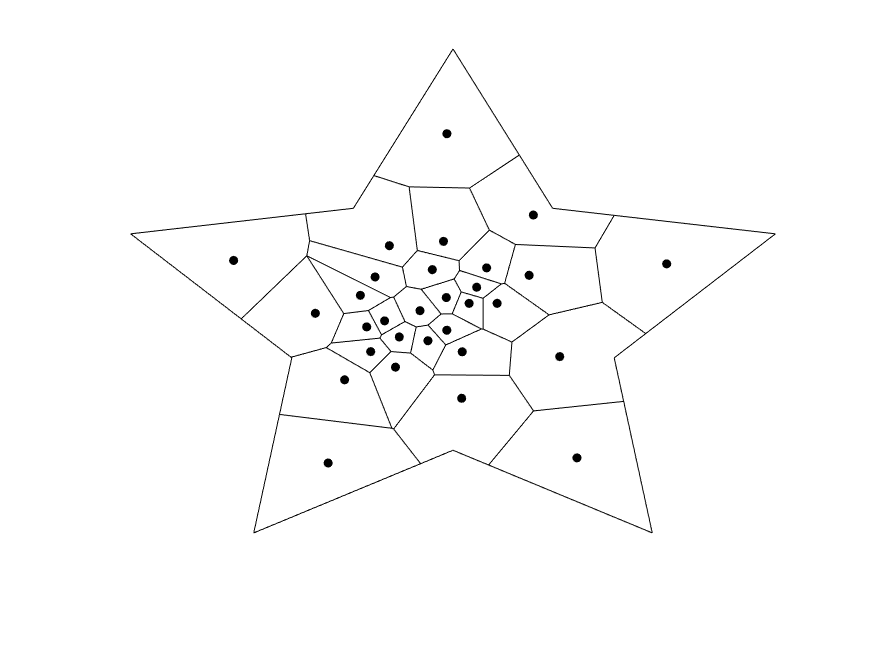
\includegraphics[width=\textwidth]{report/Images/Theory/voronoi/centroidal_voronoi_diagram_0.png}
        \caption{Random Voronoi diagram}
        \label{fig:notCVD}
    \end{subfigure}
    \begin{subfigure}[b]{0.4\textwidth}
        \centering
        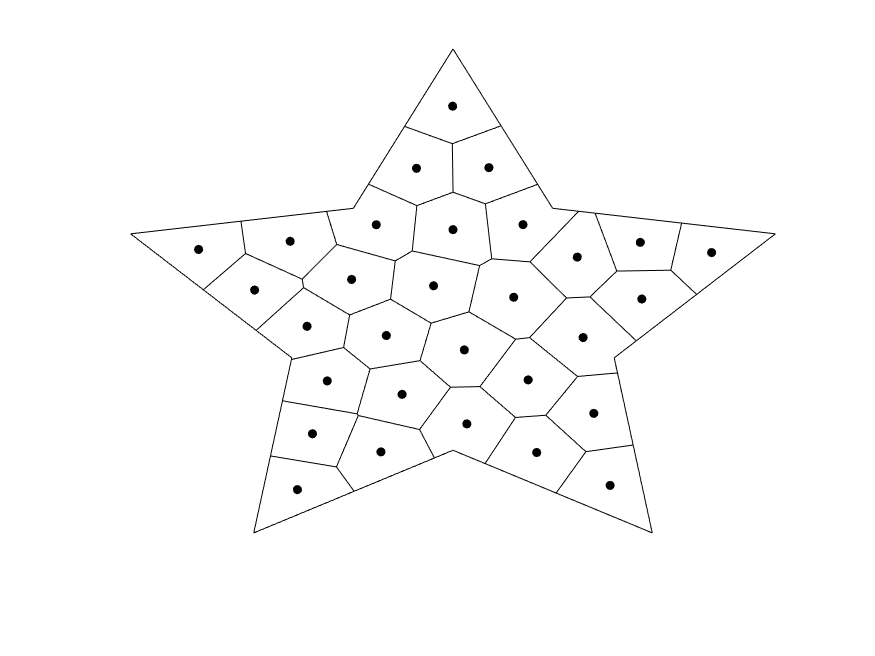
\includegraphics[width=\textwidth]{report/Images/Theory/voronoi/centroidal_voronoi_diagram.png}
        \caption{Centroidal Voronoi diagram}
        \label{fig:CVD}
    \end{subfigure}
    \caption{Comparison of centroidal and non-centroidal Voronoi diagrams}
    \label{fig:CVD_comparison}
\end{figure}

Several methods for generating CVDs exist, and one of the simplest is by using fixed-point iteration. The method, called Lloyd's method, is shown in Algorithm~\ref{alg:fixed_point}.

\begin{pseudocode}[label=alg:fixed_point]{Lloyd's method}
    Make an initial set of sites
    Until convergence:
        Construct Voronoi diagram of sites
        Compute centroids of the Voronoi diagram
        Use the centroids as new sites
\end{pseudocode}

While this method is simple and easy to implement, its linear convergence limits its usability. A quasi-Newton method is introduced by \textcite{CVDmethods}, using the CVD energy function given by
\begin{equation}
    F(x) = \sum_{i=1}^m \int_{V_i} \rho(\mathbf{y}) \abs{\mathbf{y} - c_i}^2 d\mathbf{y},
\end{equation}
which is minimized when $p_i = c_i$. This method is both faster and more robust than Lloyd's method \cite{CVDmethods}.

\subsubsection{Optimal Delaunay triangulation}
\label{sec:optimal-delaunay}
Another method for generating nice Voronoi diagrams is by exploiting the duality between Delaunay triangulations and Voronoi diagrams and using a force based algorithm. The optimal Delaunay triangulation, introduced by \textcite{Distmesh}, associates each Delaunay vertex with a joint and each edge with a spring. By defining an element size function $h(x, y)$, we attain the uncompressed length of the springs. We then let the forces follow Hooke's law, but only for repulsive forces, i.e., the force $f$ from a spring with length $l$ and uncompressed length $l_0$ is given by
\begin{equation}
    \label{eq:delaunay_force}
    f(l, l_0) = \begin{cases}
        l_0 - l, & l < l_0, \\
        0, & l \ge l_0.
    \end{cases}
\end{equation}

The total force on a point, $F(p_i)$, is simply the sum of the force from all springs connected to $p_i$. We have two special types of points to consider. Points along the border must avoid getting pushed out of the domain. To do so, we add an external force perpendicular to the border pointing inwards, balancing the internal forces. We can also have fixed joints. These are simply not allowed to move, no matter the applied force. The optimization loop, then, is simple:

\begin{pseudocode}[label=alg:delaunay_force]{Optimal Delaunay triangulation}
    Make an initial set of sites
    Until convergence:
        Calculate Delaunay triangulation of sites
        For each edge in the triangulation:
            Calculate force of the associated spring
        For each non-fixed vertex in the triangulation:
            Calculate the sum of forces on the vertex, including external forces
            Move vertex a set step length along the sum of forces
\end{pseudocode}

\subsection{PEBI grids}
Several meshing-related sources, including \cite{UPR_chapter} and \cite{UPR_thesis}, operate with what they call \emph{PEBI grids} -- PErpendicular BIsector grids. \textcite{UPR_thesis} operates with the following definition:

\begin{definition}[PEBI grid]
\label{def:PEBI-grid}
Let $P\in \mathbb{R}^n$ be a finite point set and let $\mathcal{B}$ be the PEBI grid of $P$. For each site $p_i \in P$, a cell $b_i$ is generated by the following algorithm:
\begin{enumerate}
    \item For each other site in $p_j \in P$, create the "perpendicular bisector plane" of $p_i$ and $p_j$, i.e., the plane that splits $P$ in two subspaces perpendicular to the line from $p_i$ to $p_j$, in the middle of the two points.
    \item Let $H(p_i, p_j)$ be the subspace that contains $p_i$.
\end{enumerate}
The cell $b_i$ is then defined as the intersection of all these subspaces, i.e.,
\begin{equation}
    b_i = \bigcap_{p_j \in P \setminus p_i} H(p_i, p_j).
\end{equation}
\end{definition}

This process is visualized in \autoref{fig:PEBI-definition}, in which $p_i$ is the site marked by a red dot, with blue dots representing the other $p_j \in P$. The dashed lines are the lines from $p_i$ to each $p_j$, with the solid black lines representing the two dimensional perpendicular bisector planes between $p_i$ and each $p_j$. The light-red area is the cell $b_i$.

\begin{figure}[ht]
    \centering
    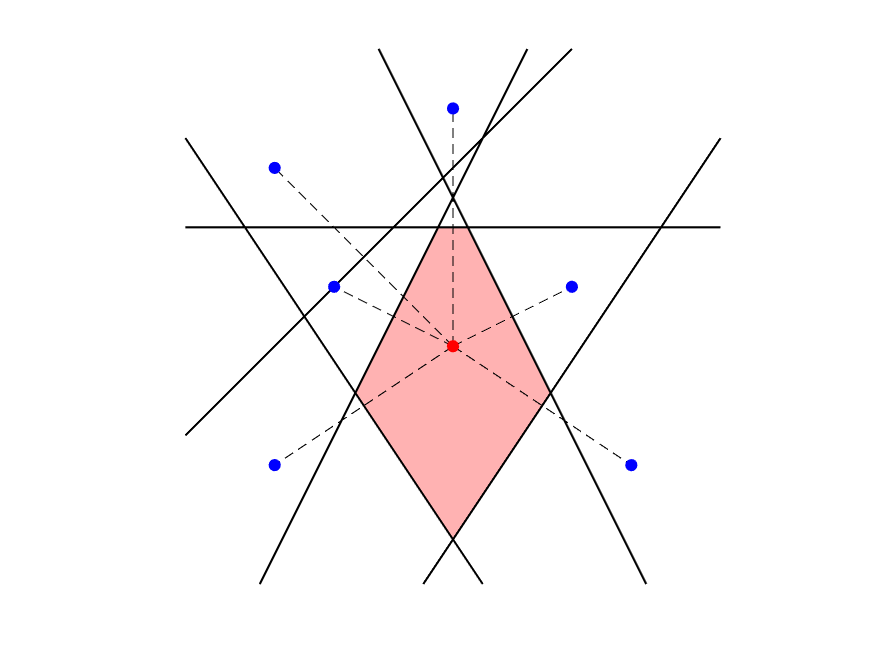
\includegraphics[width=0.7\textwidth]{report/Images/Theory/PEBI_definition.png}
    \caption{Visualization of PEBI generation.}
    \label{fig:PEBI-definition}
\end{figure}

Looking at the cell marked in \autoref{fig:PEBI-definition}, it appears to resemble the central Voronoi cell in \autoref{fig:ex:voronoi-voronoi}. In fact, \textcite{UPR_chapter} present proof that PEBI grids are Voronoi diagrams, which we repeat here for completeness.

\begin{theorem}
\label{theorem:PEBI-voronoi}
Let $P$ be a finite point set, $P \in \mathcal{D}$. Let $\mathcal{B}$ be a PEBI grid of $P$. Then $\mathcal{B}$ is a Voronoi diagram of $P$.
\end{theorem}
\begin{proof}
First look at a randomly selected point $x \in \mathcal{D}$. As every point in $\mathcal{D}$ belongs to at least one Voronoi cell, assume $x$ belongs to cell $v_i$ in the Voronoi diagram of $P$. We know from  \autoref{eq:clipped-voronoi} that $x$ is at least as close to $v_i$ as any other $v_j$. This means that $x$ will be in the subspace $H(p_i, p_j)$ for all $j$, meaning it must be in the intersection of all $H(p_i, p_j)$. It thus follows from Definition \ref{def:PEBI-grid} that $x \in b_i$.

Now, assume that $x$ belongs to PEBI cell $b_i$. This means it is part of all subspaces $H(p_i, p_j)$, and thus must be at least as close to $p_i$ as any other $p_j \in P$. As this holds for all $j$, it follows from \autoref{eq:clipped-voronoi} that $x \in v_i$.

We thus have $x \in v_i \iff x \in b_i$, thus $v_i = b_i$ and PEBI grids are Voronoi diagrams. The proof also holds for unclipped Voronoi diagrams.
\end{proof}

As PEBI is widely used in the literature, as well as in the software used for this thesis, I will use the term PEBI grids, rather than Voronoi diagrams, going forward.

